\documentclass[a4paper,8pt]{article}
\usepackage[utf8]{inputenc}
\usepackage[left=1cm,right=1cm,top=1cm,bottom=1cm]{geometry}
\usepackage{graphicx}

%opening
\title{AG44 Project 1 - Ariadne's Thread}
\author{Pierre RUFFY}

\begin{document}

\maketitle

\section{Introduction}
The objective of the project is to learn how to manipulate a graph. We receive an adjacency matrix that represent the connections between the different 
area's of the game and must create a graph and obtain the different strongly connected component of the graph (the levels). For example :

\begin{figure}[h]
\centering
 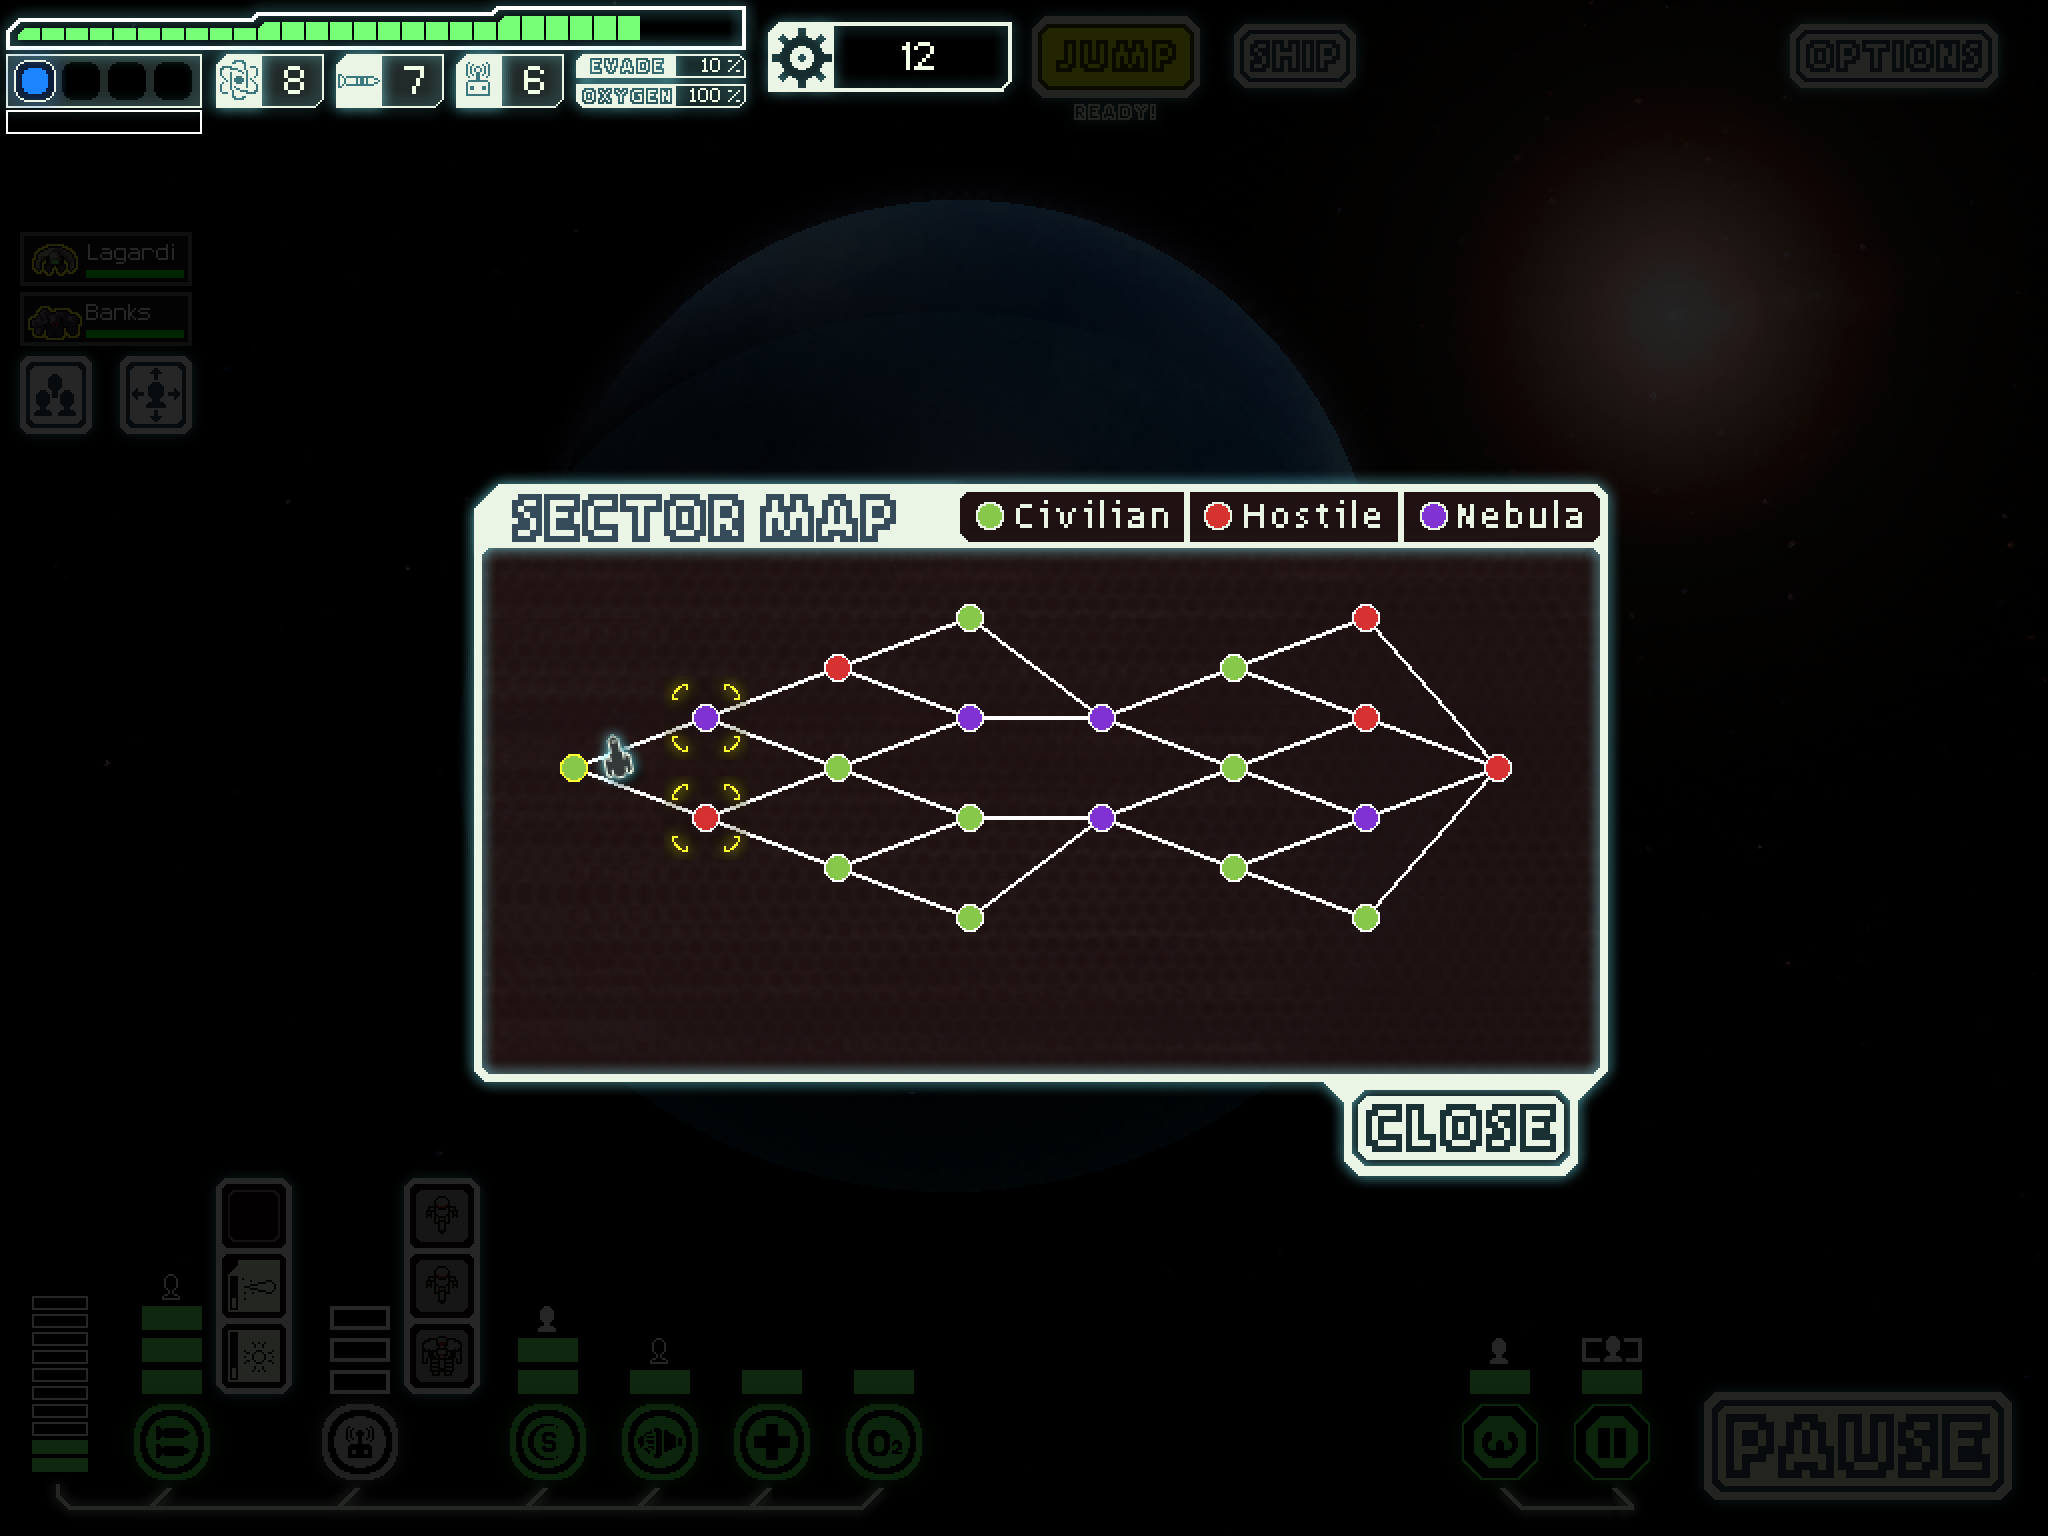
\includegraphics[scale=0.1]{ftl-mapoflevel.png}
\caption{FTL - Graph of Level}
\end{figure}

This image show us the graph of the level in the game. Each level is composed by a lot of area but it's not shown in the level graph\\

\begin{figure}[h]
\centering
 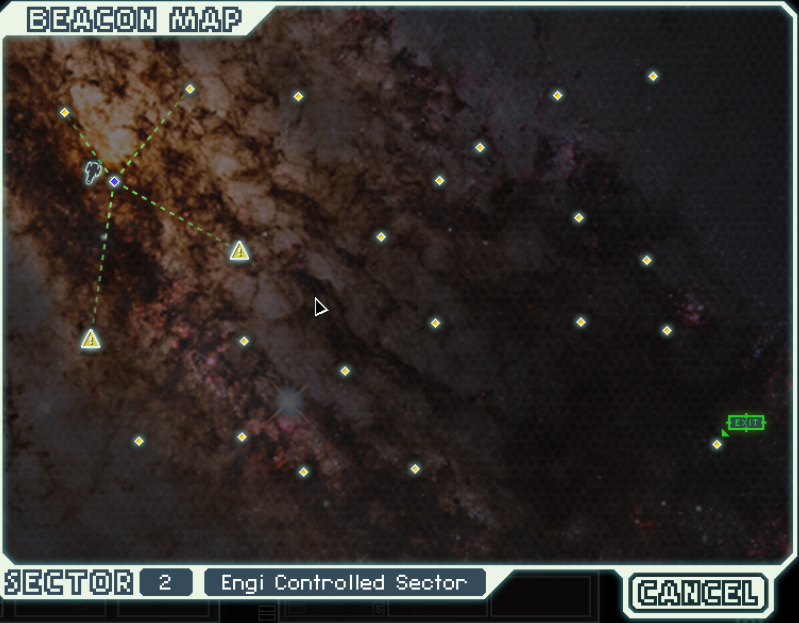
\includegraphics[scale=0.3]{ftl-level.png}
\caption{FTL - Level Content}
\end{figure}
Here we can see the content of the level. This game is a good example for representing this project because the main objective is to going from the first level 
(on the left of the first image) to the last. During the traversal of each level the players must take a path the longest possible to obtain the greatest reward 
possible and upgrade his ship. Although he have more restriction that just searching for the longest path.
\section{Implementation}
\subsection{The language}
For implementing the graph i choose the python. The reason of this choice was simply because i've got, with this project, the oppurtunity to learn this language. 

\subsection{Representation of the graph}
In order to represent the graph i have deciced to create a class graph. This class is composed by a list of integer that represent the vertices and a list of list 
for the neighbours. I've tried before to make a class vertex and edge but didn't succed to use them properly so i came back to this representation.

The graph is also composed by three other list. The list call ``levels''. It's a list of the level that work like the list of vertices. The list ``levelContent'' 
this list contained others list. Each list is the content of a level, in other word the different area in each strongly connected component. Finally a list for the 
neighbours of each level.

\subsection{Creation of the graph}
The creation of the graph take two step. First we read an adjacency matrix in a text file.  The matrix is stored in a list of list where each list reprensent a line. 
After reading the matrix we create the graph by parsing the data we received. Each line correspond to a new node. And for each line if we read a 1 then we add the indices 
in the neighbours list associated to the line we are currently reading.

\subsection{Determining the level}
For determining the strongly connected component of the graph i used the tarjan algorithm. The algorithm is recursive and visit every node of the graph once. For
that we created three lists. One that store all the node already visited one that store the indew of the lowest node accessible and a stack. When we start the 
algorithm we look the son of the vertices. If it haven't been visited yet we called the function to visit the son. If the son has been visited before we look if he 
is in the stack. If it's the case we change the index by the one of the son in the lowest index list. If the lowest index of a vertex is his index then we've got an 
element of a strongly connected component and we pop the stack.

\subsection{Test}
When we run the program with the matrix given we obtain this solution :


The graph is

[1, 2, 3, 4, 5, 6, 7, 8]

[[2], [3, 4], [2, 5, 7], [5, 8], [4, 8], [2, 8], [6, 8], []]
 
Adjacency matrix of the levels 

[0, 0, 0, 0]

[2, 0, 0, 0]

[2, 2, 0, 0]

[0, 0, 1, 0]
 
List of levels :

[1, 2, 3, 4]
 
Content of each levels : 

[[8], [4, 5], [2, 3, 6, 7], [1]]
 
Neigbours of each levels :

[[], 1, 2, 3]


\end{document}
